\documentclass[twocolumn,10pt]{asme2ej}
\usepackage[utf8]{inputenc}
\usepackage[
	backend=biber,
	style=numeric
]{biblatex}
\addbibresource{../bibliography.bib}
\usepackage[dvipsnames]{xcolor}
\usepackage{csquotes}
\usepackage{url}
\usepackage{graphicx}
\graphicspath{{../images/}}
\usepackage{booktabs}
\usepackage{hyperref}
\hypersetup{
	colorlinks=true,
	linkcolor=blue,
	urlcolor=blue,
	citecolor=blue,
}
\usepackage{comment}
\usepackage{epsfig}

\title{Rethinking Model Architecture and Means of Delivery to get Video Interaction with Generative Neural Networks Online}
\date{\today}
\author{Josh Murr}

\begin{document}

\pagenumbering{gobble}
\maketitle
% \newpage
% \pagenumbering{arabic}
% \tableofcontents
% \newpage

\begin{abstract}
	% 250 Words
	The lines between scientific researcher and artist are continually being blurred as artists adopt machine learning methods\cite{anna_ridler}, or researchers apply their tools in novel and interesting ways\cite{deep_dream_guy} rethinking how cutting-edge research can be applied to create image generation tools or interrogate the tools themselves. \textit{Learning to See} by Memo Akten\cite{lts_memo} is one such seminal artwork which does both. Reframing the tools which we are in fact living with day-to-day in the context of the gallery provides an opportunity to think deeper about how a neural network interprets the data it is given and to witness the capabilities and limitations of such a system. \textit{Learning to See} in particular has a uniquely simple interaction allowing the visitor to play with the network in real time. This work shows that simply shrinking the Pix2Pix\cite{1611.07004} model which powers \textit{Learning to See}, and a custom made WebGL wrapper for TensorflowJS to make a pipeline more suited to video achieves useable results when served online, even on commonplace integrated graphics processing units. This brings the unique interaction developed by Akten \textit{et al}\cite{2003.00902} into the homes of many people and offers exciting possibilites to future video based interaction with machine learing on the internet. The work is currently online here: \url{https://learning-to-learn-to-see.netlify.app/}, and code available here: \url{https://github.com/joshmurr/cci-pix2pix-demo/}.
\end{abstract}

\begin{figure}[h!]
	\begin{center}
		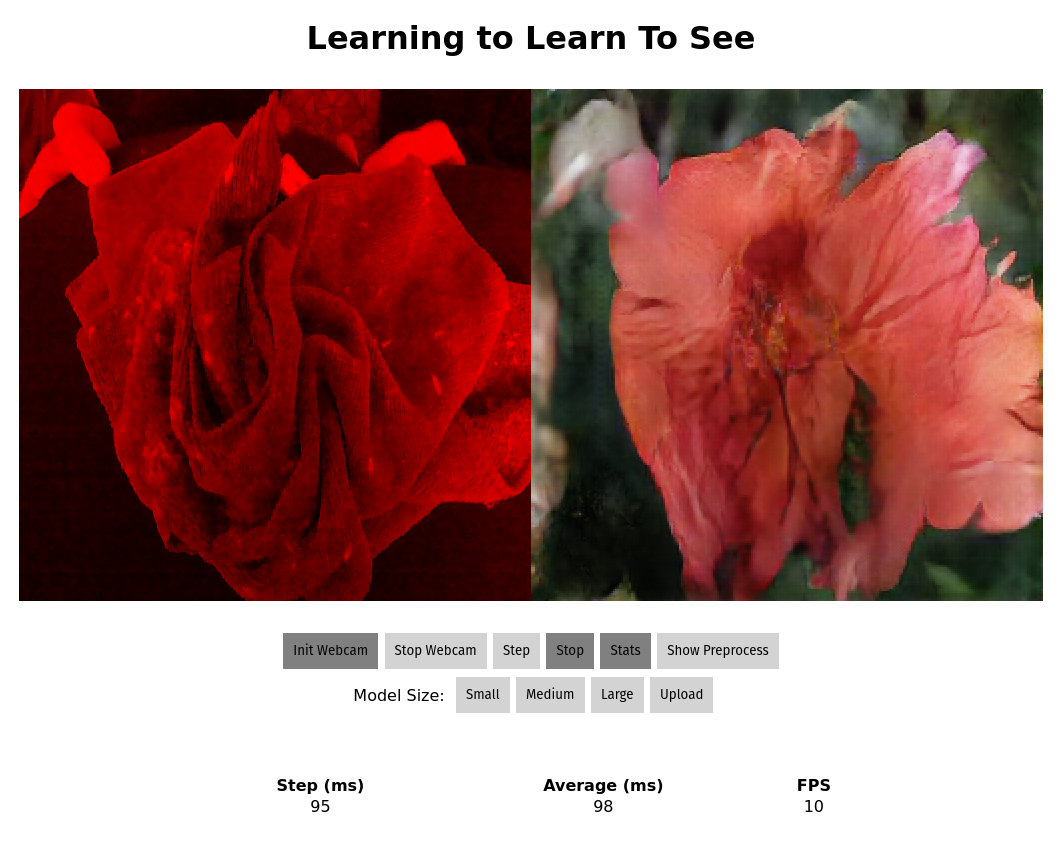
\includegraphics[width=\columnwidth]{ltlts_online2}
	\end{center}
	\caption{The online platform running the largest model trained on the \textit{102 Category Flower Dataset}\cite{flowers_dataset} for 250 epochs.}
\end{figure}

\section{Introduction}
% 500 Words
% --- 568 WORDS ---
Machine Learning (ML) is a part of our everyday lives. For the technical among us it is currently easy enough to see the patterns in the outputs of these black-box systems---as the end of our sentence is predicted as we type, or an item we did not know we wanted is offered to us as we shop. There are however many non-technical users of ML systems who can only see the black-box, or perhaps nothing at all; as Arthur C. Clarke famously said \textit{``Any sufficiently advanced technology is indistinguishable from magic.''}\cite{toffler_1972} It is often the case that exciting new technologies are adopted by artists as readily as industry because the gallery provides a unique environment to present back the to the user one of these black-boxes in a drastically different context. Artists such as Mario Klingemann\cite{mario_klingemann}, Terence Broad\cite{terry_broad} or Anna Ridler\cite{anna_ridler} are all excellent examples of artists who have done just this.

\textit{Learning to See} by Memo Akten\cite{lts_memo} is another example, but unique in its own way in that it gives the user an interactive experience of the artwork; an immediate image translation of arbitrary objects placed on a tabletop to a rich image of waves crashing, the night sky or ever changing flowers. The user is able to manipulate the input data and witness how the model interprets this to produce an output image in front of them. Although the model still exists as a black box, being able to see how input-affects-output in real time is extremely powerful.

\begin{figure}[h]
	\centering
	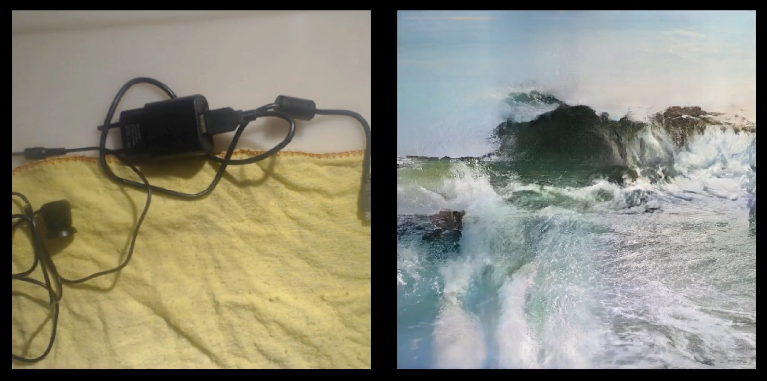
\includegraphics[width=\columnwidth]{lts_still}
	\caption{A frame from Learning to See using a model trained on ocean waves. --- \copyright Memo Akten,2017}
\end{figure}

Witnessing the relationship between input and output is in many ways more vital to understanding the function of a Neural Network (NN) than understanding what a neuron is and how backpropagation works. The role of the artist is important here as these artworks have done a huge amount to shed light on dataset bias\cite{crawford_paglen_2019}, stimulate conversation about ownership and copyright\cite{romano_2016} and show both the capabilities of ML systems \textit{and} the limitations. It is therefore of great importance to make these stimulating artworks accessible to many more people, which is not as simple as it might seem.

Unfortunately the gallery in itself is a black box to many, entry restricted by a fee or simply by the location of the gallery. Moving such interactive experiences online is a clear next step as once something is online it is immediately available to anyone with an internet connection --- this then poses numerous challenges. Even a modestly sized NN can contain many millions of parameters. Modern computers are able to perform millions of floating point operations per second (FLOPS) but advances in ML research have shown that \textit{deeper} models and more data produces better results\cite{2005.14165}; as such, without expensive hardware acceleration from discrete graphics processing units (GPU) or even more modern tensor processing units (TPU), an average modern computer cannot crunch the numbers needed to run a large, deep NN\@. Even if one \textit{could} perform the necessary FLOPS, storing this number of parameters can take up gigabytes of memory and so downloading the weights and biases of a pre-trained model can be a time consuming process detracting from the real-time focus.

This paper aims to explore each of these challenges and to look at each through the perspective of the artworks previously described with the aim of getting a piece like \textit{Learning to See} online and useable by most with access to the internet.


\section{Background Context}
% 500-1000 Words
% --- 891 WORDS ---

Getting NNs working online and on the clients machine is not a new thing and with modern CPUs it has certainly been shown possible to train and run a simple enough model in the browser\cite{karparthy_conjs_2016, brainjs, synaptic, mind, kerasjs} and many tools exist which aim to visualise the architecture of a model and show the training process\cite{broad_cnn_vis_2016, tensorflow_playground, 1704.01942}. Such tools are invaluable as learning resources for those dedicated to learning about machine learning. However they are often tailored to that use-case expecting the user to have higher motivation for understanding the process, more than the average online `passer-by'.

There is an increasing number of tools available online which use an interactive machine learning approach allowing the user to retrain a model in real-time to create unique interactions of the users specification\cite{magenta, mimic, teachablemachines}. Again this is valuable work and useful to many, but often requires active engagement from the user and some knowledge of the process.

\textit{Learning to See} provides an instinctive way for the user to interact with machine learning, avoiding technical terms or a prerequisite knowledge which is simply not seen online (at the time of writing). This is largely down to the issues described above, and these are especially applicable to image generative models which will be discussed further below.

\textit{Learning to See} is an adaptation of the Pix2Pix model\cite{1611.07004} which is a Conditional Generative Adversarial Network (cGAN)\cite{1701.00160}. Unlike a conventional GAN\cite{1406.2661}, a cGAN takes in two data samples as input, in the case of the Pix2Pix model it is a \textit{target} image and an \textit{input} image. Pix2Pix also learns a structured loss which means it is able to penalize any possible structure that differs between output and target\cite{1611.07004}. This model architecture is extremely flexible and has been shown to be useful for many use cases as detailed in the original paper. However neither the original Pix2Pix paper nor \textit{Learning to See} had an incentive to create a small model; a good result is simply a sharp image with a predictable output from a given input. As stated by the Pix2Pix authors measuring the results of an image generating GAN is an open issue\cite{1606.03498, 1611.07004} and in an artistic context quantifiying the outcome is largely pointless --- a good result is one which delivers the message of the artist.

It is worth noting that other generative models of similar architecture to Pix2Pix have been developed since, notably CycleGAN\cite{1703.10593} and GauGAN\cite{1903.07291}. However these models are also significantly more complex and did not seem conducive to a lightweight and performant system with the given requirements. Image generative models are notoriously unstable in training, intuition (and Jonathan Hui) notes that it is easier to recognise an image than it is to create one\cite{hard_to_train_gans}. Therefore traditional NN compression\cite{2006.03669} is often unsuited to GANs. There has been work in GAN compression which has yielded impressive results, but it is a quite esoteric, unconventional compression involving programmatically finding alternate model architectures with neural architecture search (NAS) and teacher--student model pairing to distill knowledge into a smaller architecture\cite{2003.08936}. Simplicity was the first port-of-call for this work thus methods shown in the aforementioned works remain untested in this context for now.

Designing and training a NN is of course not limited to the big name ML frameworks like Tensorflow\cite{tf} or PyTorch\cite{pytorch}, but given the modular nature of a NN and the want in most cases to utilise the GPU for faster training and inference, it is no surprise that a limited number of ML frameworks have become the go-to to create and iterate on a novel ML model and to take care of interfacing with a highly optimized backend and the GPU at a lower level. Tensorflow offers a relatively full end-to-end pipeline from designing and training a model in Python, to saving and converting a model into something can be run in the browser using TensorflowJS\cite{tfjs}. A trained model is simply a collection of weights and biases and to use this model on a different device or context, these weights and biases need to be loaded into a model of the same architecture as was used to train the model. The pipeline from training-to-browser is largely about keeping data structures in order and consistent such that the next process knows how to work with it. As part of the process Tensorflow has developed the TensorflowJS Converter\cite{tfjs_converter} which converts a saved model into a a series of binary files which hold the weights and a \verb|.json| file which is the blueprints of the model. When uploading a model TensorflowJS dynamically creates a succession of routines in the chosen backend (WebGL, WebAssembly, WebGPU, etc.) to take care of specific tasks such as 2D convolutions, batchnorm, max pooling etc.%  Moving data through the computational graph is now the difficult part as each of these stages exists as a discrete routine which performs efficient calculations, but getting the data out of the GPU to pass on to the next program comes at a great performance cost and increases latency of the overall system, particularly with web technologies\cite{optimizing_webgl}.

There exists nothing even similar to \textit{Learning to See} in the catalog of examples provided by TensrflowJS --- i.e.\ a model which takes video as input and produces video as output. Thus the uniqueness of this use case has yielded a number of hurdles to overcome to achieve something usable on the web for \textit{most users} (users with a reasonably modern laptop, produced in the past 5 years).


\section{Method}
% 500-750 words - how you will approach the problem
% (use well understood methods and don’t roll your own)
% mixed methods fine (quantitative - data and qualitative - surveys, viewpoints)
% --- 892 WORDS ---
TensorflowJS is currently the most developed framework for deploying models in the browser so working with the Tensorflow pipeline made the most sense. The model for this work was based on the Tensorflow implementation\cite{tf_p2p} and adjusted according to the \textit{Learning to See} paper: the input and target images are the same, only the input goes through a series of augmentations, details of which can be found in the original paper\cite{2003.00902}.

The data augmentation requires the generator to take a single channel input. Augmenting the dataset at runtime during training makes forming a dataset very easy as in reality a full dataset is simply a directory of many similar images. As stated earlier, evaluating the model quantitatively by some distance metric has been shown to be of little use, and particularly in this case the quality of the outcome can only really be measured by how well it performs when interacted with. Thus the common process of splitting a dataset into \textit{training} and \textit{testing} data at a 4:1 split was not as important; however approximately 5\% of the dataset was reserved for testing after training for visual inspection.

\begin{figure}
	\centering
	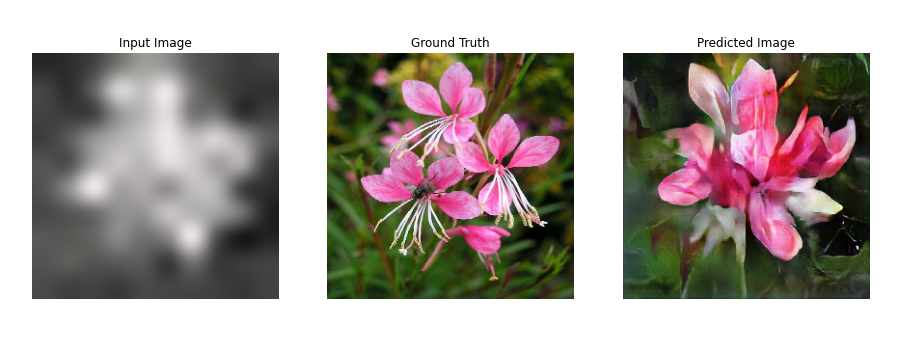
\includegraphics[width=\columnwidth]{250_epochs}
	\caption{The output of a `large' model trained on the \textit{102 Category Flower Dataset}\cite{flowers_dataset} for 250 epochs.}
\end{figure}

It was found that for a model that takes an input image size of 256$\times$256 pixels and produces an output of the same size, a dataset of 800--1000 images uniformly shuffled with a batch size of 4 was sufficient to produce \textit{interesting} results --- in this case \textit{interesting} means: varied enough to provide unique experiences whilst producing a output which is representative of the input data. Differences between the model sizes can be seen in \ref{table:model_details}. The models were trained on a NVIDIA Quadro RTX 6000 with 24GB memory locally, or a Tesla P100-PCIE with 16GB memory using Google Colab. In either case a usable model will train in a few hours allowing for a relatively quick development cycle. %More details on the training process and some tools developed to make the process easy and fast in appendix \ref{appendix:training}.

The Pix2Pix generator is an Autoencoder similar to the ``U-Net'' architecture\cite{1505.04597} but differs in some key ways, and we offer some further changes to drastically reduce the size. The generator consists of 8 2D convolution layers downsampling the input data in width and height, and 7 transpose convolutions upsampling the data back to original size. Each layer is batchnormalized\cite{1502.03167} apart from the first, and layers 8--10 have dropout\cite{JMLR:v15:srivastava14a} applied at a rate of 50\%. The Pix2Pix architecture includes no avg- or max-pooling as all filter kernels are 4$\times$4 and a stride of 2 is used. This has the effect of downsampling the layer input by half in width and height, thus circumventing the need for any kind of pooling, otherwise known as an \textit{all convolutional net}\cite{1412.6806}. The difference proposed in this work is to greatly reduce the number of filters used in each layer. The majority of trainable parameters are found in the middle of the generator as a result of the structure described. By reducing the number of filters in each layer by up to a factor of 8, very usable results were obtained whilst drastically reducing the model size --- more discussion on the impacts of a smaller model are found in Results.

\begin{small}
	\begin{table}
		\begin{center}
			\begin{tabular}{p{2cm}p{2cm}p{2cm}p{2cm}}
				\toprule
				Generator Layer & Pix2Pix & Our Small & Our Medium \\
				\midrule
				1               & 64      & 4         & 8          \\
				2               & 128     & 8         & 16         \\
				3               & 256     & 16        & 32         \\
				4               & 512     & 32        & 64         \\
				5               & 512     & 64        & 128        \\
				6               & 512     & 128       & 256        \\
				7               & 512     & 256       & 512        \\
				8               & 512     & 512       & 512        \\
				9               & 512     & 256       & 512        \\
				10              & 512     & 128       & 256        \\
				11              & 512     & 64        & 128        \\
				12              & 512     & 32        & 64         \\
				13              & 512     & 16        & 32         \\
				14              & 256     & 8         & 16         \\
				15              & 128     & 4         & 8          \\
				\bottomrule
			\end{tabular}
			\caption{Number of filters per layer in the generator. TODO: Replace table with graphic of model architecture, showing difference between model sizes.}
		\end{center}
	\end{table}
\end{small}

Once a model is trained, it is saved using the \verb|HDF5| format (\verb|.h5|) and converted using the TensorflowJS Converter. The Converter provides options for compressing the model of varying levels of severity. It was found that the compression of the model:

\begin{enumerate}
	\item Does a great deal to reduce the size (in memory) of the model.
	\item Does very little to improve performance in inference.
	\item Does very little to affect the output of the model.
\end{enumerate}

Therefore the highest compression of \verb|uint8_affine_quantize| can be used to reduce the size by 4$\times$, while maintaining only a very slightly compromised output.

Finally, a bespoke WebGL wrapper consisting of a number of shader programs was created to handle the input data (pre-augmentation to match that in training) and the output data to render the image to the screen as video. It was found that the image handling capabilities of TensorflowJS seem to be tailored to static images. In inference, the data is of the \textit{tensor} data structure and is transformed and manipulated by the model, but at each iteration of the draw cycle a frame of video must be preprocessed and then converted into a format which can be digested by the model, and then the output of the model must be converted back into a data structure which the browser can handle to display as an image, or in our case, video. The internal computation at inference is handled by WebGL shader programs compiled by TensorflowJS, but the input/output was a rather slow process of converting the tensor data back to pixels value-by-value. The input shader programs receives data from the webcam as a 16$\times$16 image and scales it up to 256$\times$256 while applying three gaussian blurs --- slightly different to the training process but the effect is the same. The data is extracted using \verb|<WebGL>.readPixels()|, converted to a tensor object and passed to the model to process. The output of the model is a tensor object but already of the structure of a 3-channel image as a result of the architecture of the model itself. The data is easily extracted as a 32 bit float array and passed into a very simple shader program as an RGB texture to be rendered to a canvas element in the browser.

\begin{comment}
It can be observed in the stack trace (using the developer tools of most modern browsers, in this case Firefox and Chrome were used) that TensorflowJS is still having to do a lot of the working moving data around and reshaping data in Javascript, while the heavy computation is deferred to shader programs. This moving data around comes at a great cost which is felt particualrly in the case of video based interaction. As a slight aside, a `pure' WebGL Autoencoder of the same stucture as the Pix2Pix generator was created simply to perform the same number of calculations in the same fashion to compare performance, and to give a glimpse into a novel approach to machine learning online which is perhaps more streamlined.
\end{comment}

\section{Results}
% 500-750 words
% -- 389 WORDS ---

\begin{figure}[h]
	\centering
	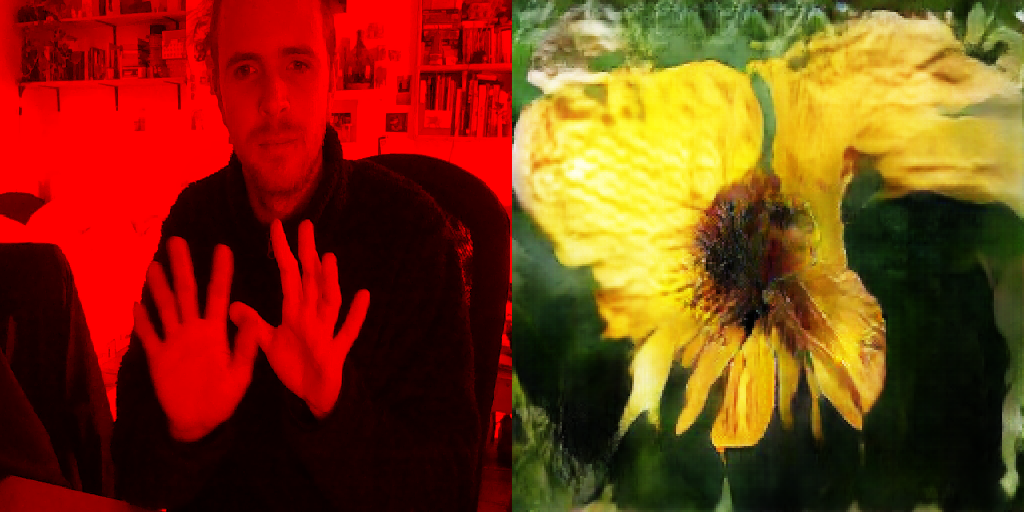
\includegraphics[width=\columnwidth]{00}
	\caption{The large model in use running on an NVIDIA RTX 2070.}
\end{figure}

A test-bed was created with the aforementioned processes to test three sizes of model. The project is currently online at \url{https://learning-to-learn-to-see.netlify.app/}. % In the table below \textit{Avg Step Time} is the time taken to create a new frame to output which includes pre-processing and post-processing via the custom WebGL wrapper.

\begin{table}[t]
	\begin{center}
		\begin{tabular}{ccc}
			\hline
			Model  & HDF5 Size (mb) & Uint8 Compressed Size (mb) \\
			\hline
			Small  & 25.3           & 6.3                        \\
			Medium & 67.3           & 16.9                       \\
			Large  & 217.8          & 54.5                       \\
			\hline
		\end{tabular}
		\label{table:model_details}
	\end{center}
\end{table}

%Small  & 25323104           & 6365943 
%Medium & 67280248           & 16852241
%Large  & 217835560          & 54484213


As already stated, the focus was on finding a sufficiently responsive interaction for the user while maintaining enough variety in the output to maintain engagement. The target audience is someone with a relatively modern computer and not necessarily someone with a computer with a high specification GPU. For testing the user is able to download a model size at their choosing or upload their own, and different statistics are displayed.

In the table below \textit{D-GPU} means \textit{Discrete-GPU} and \textit{I-GPU} means \textit{Integrated-GPU}. \textit{FPS} is rounded to the nearest number. All figures are taken from the online platform.

\begin{small}
	\begin{center}
		\newcolumntype{b}{>{\raggedright\arraybackslash\hsize=0.65\hsize}X}
		\newcolumntype{s}{>{\raggedleft\arraybackslash\hsize=0.15\hsize}X}
		\begin{tabularx}{0.8\textwidth}{bsss}
			\toprule
			\multicolumn{4}{c}{Performance (FPS) on Various Computers} \\
			\toprule
			Machine                     & Small & Medium & Large       \\
			\midrule
			System76 Laptop 2020, D-GPU & 50    & 41     & 10          \\
			System76 Laptop 2020, I-GPU & 26    & 12     & 0           \\
			Macbook Pro 2020, I-GPU     & 25    & 15     & 1           \\
			Macbook Pro 2017, D-GPU     & 40    & 27     & 0           \\
			Macbook Pro 2017, I-GPU     & 26    & 14     & 0           \\
			Macbook Pro 2015, I-GPU     & 30    & 18     & 0           \\
			Macbook Pro 2015, D-GPU     & 27    & 18     & 1           \\
			MSI Laptop 2016, I-GPU      & 18    & 12     & 1           \\
			Pixel 3A Phone              & 3     & -      & -           \\
			Samsung Galaxy A20e Phone   & 4     & -      & -           \\
			\bottomrule
		\end{tabularx}
	\end{center}
\end{small}

In general the results are very promising. The average frame rate on an integrated GPU is $\sim$14FPS which suggests that the average `everyday' computer will be able to run the \textit{medium} sized model at a useable speed while a gaming-laptop with a discrete GPU can observe good results even on the largest model.

It can be observed that models trained with fewer parameters struggle to generalise. The \textit{102 Category Flower Dataset}\cite{flowers_dataset} has proven to be a useful dataset for testing as it is quite varied; the subject is not always centered in the image, the colours vary drastically and there is great variation in tone and texture throughout. A full sized \textit{large} model is capable of capturing a lot of this texture, however with fewer filters in the smaller models, artefacts of the kernels themselves often appear in the output, as seen in Figure ~\ref{fig:kernelsInOutput}.

\begin{figure}[h!]
	\centering
	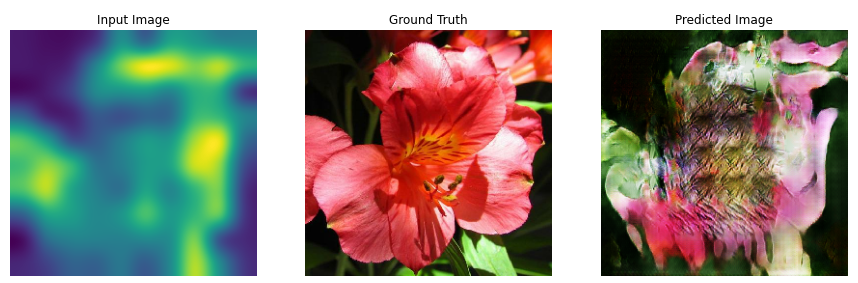
\includegraphics[scale=0.3]{artefacts}
	\caption{A medium model trained for 200 epochs on the \textit{102 Category Flower Dataset}\cite{flowers_dataset} showing artefacts of the inner filters, perhaps evidence of overfitting given the smaller model size.}
	\label{fig:kernelsInOutput}
\end{figure}


In training the model is attempting to learn a mapping from a blurry greyscale image to a well defined 3-channel image. As a user interacts using the online platform one can quickly see the effects of bright or dark areas of such an abstract input, the model appears to associate these bright spots with key areas of interest in the output.

With all this in mind one can train a model with a less varied dataset (such as daytime clouds) which still produces compelling results even in the smallest model as the model needs to generalise less. A dataset produced from a timelapse of the Aurora Borealis was used for the smallest model. The smallest model does not produce particularly exciting results, but still does a good job of illustrating the relationship between input and output, and has even been shown to work on mobile devices.

\begin{figure}[h!]
	\hspace*{-0.725in}
	\centering
	\begin{tabular}{cccc}
		\subfloat{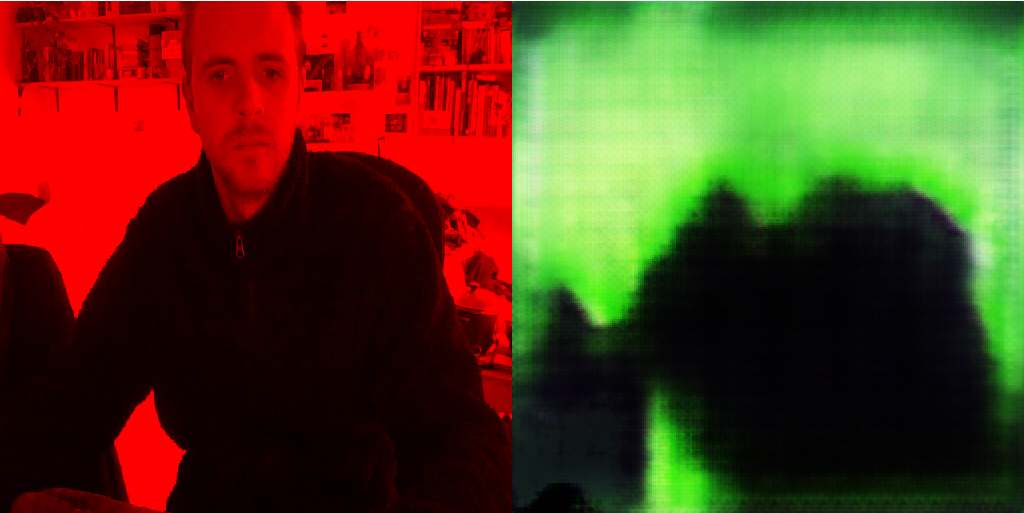
\includegraphics[width=1.5in]{aurora1}} & \subfloat{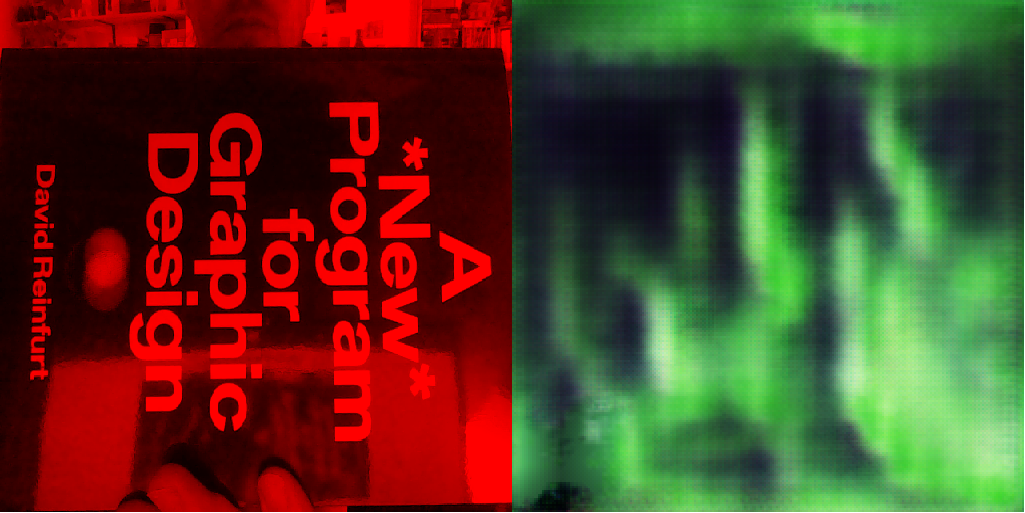
\includegraphics[width=1.5in]{aurora2}} &
		\subfloat{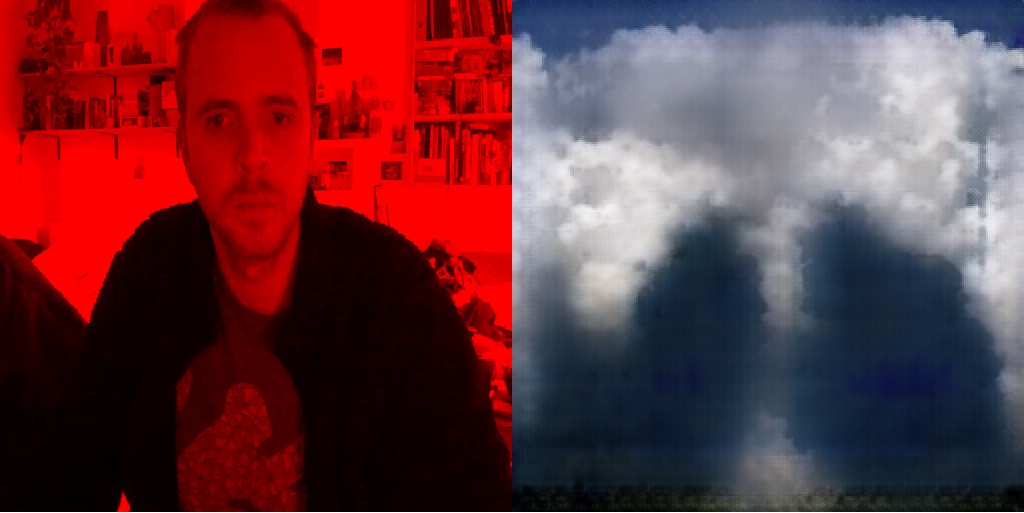
\includegraphics[width=1.5in]{clouds1}} & \subfloat{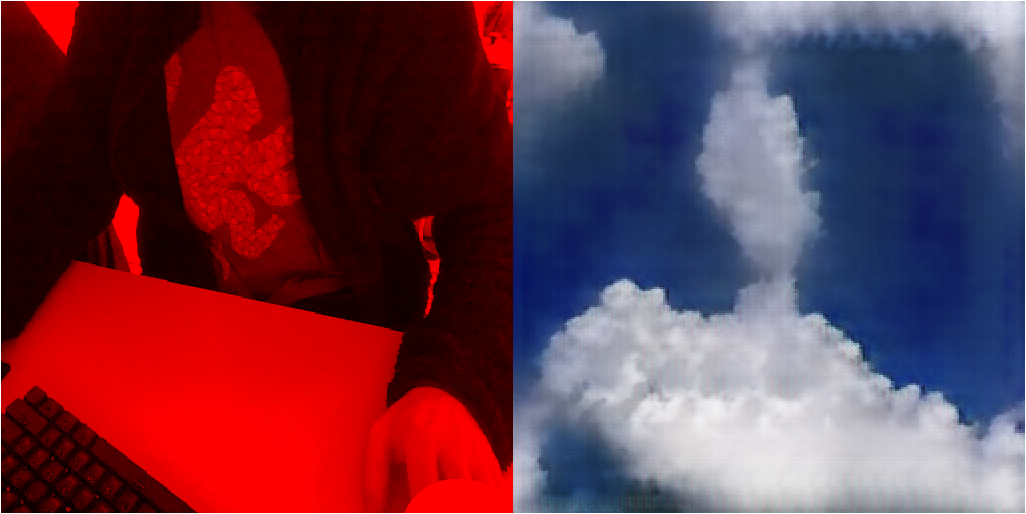
\includegraphics[width=1.5in]{clouds2}}   \\
	\end{tabular}
	\caption{Small model trained on images of Aurora Boreals (left), medium model trained on images of clouds (right).}
\end{figure}



\begin{comment}
The aforementioned `pure' WebGL Autoencoder is a scalable CNN framework which holds the core functionality to perform the forward pass of an \textit{all convolutional} network, such as that of the Pix2Pix generator.
\end{comment}


\section{Discussion}
% As long as you can cope with
The adoption of ML research into the art world offers a reframing of the application of ML research, which in turn reframes the approach to research itself. The U-Net style, all convolutional network used for the generator in the Pix2Pix model is a particularly graceful NN which at its core is \textit{only} a series 2D convolutions (omitting batchnormalisation and skip connections). This work shows that the network itself need not be complex or large to still produce results which are useable, visually interesting and accessible. As stated, if this work reaches and excites people who previously saw generative ML as off limits, then it is considered a success. Beyond that this work could lead to the development even more artistic tools in the same way that ML5\cite{ml5}, RunwayML\cite{runway} and Wekinator\cite{wekinator} have become tools for experimentation among artists and creators.

Given the smaller scale model with this workflow, the development process becomes faster and less daunting, allowing one to engage with the entire process more fully. Neural networks as a \textit{tool}, just like a paintbrush or a camera, is an exciting future in art. The iterative process involved in this work meant creating many datasets and training many models and assessing the outcome qualitatively, this helps develop a sense of \textit{how the model will react to a certain dataset}, and equally an \textit{intuition of the output}. The ability to iterate quickly is how, as a practitioner or an artist, one develops an intuition of ones tools and thus how one learns to control the medium --- a painter is not born with the ability to accurately mix color and control a brush, but it is learnt and honed over time.

This work is not only about creating art, or tools for artists. Democratising the process from start-to-finish is important to making the process accessible to all. We currently live with machine learning and artificial intelligence; as there appears to be no limits to the possibilities there is no doubt that it will find its way into even more aspects of our lives. Therefore it is imperative that the field of machine learning becomes more accessible and transparent. The first automobile was met with distrust[\emph{*find citation}] and seen as magic, the hope of this work is to dispel some myths of ML by giving the user their first ride in the car.

\begin{comment}
Given the remit of simplicity, an \textit{all \underline{WebGL} convolutional network} was created to mimic the structure of the Pix2Pix generator which shows a possible future of NN deployment on the web, specifically with video interaction in mind. All data is stored and processed in data structures suited to 2D textures which are quickly read and written to by GLSL shader programs.
\end{comment}


\section{Conclusion}
% Sum up what you have learned and where we should go next
The goal of this work is to inspire intrigue and excitement in users to take up ML as a new tool in their creative toolbox, as much as it is a fun interaction. The feedback from this work has been positive but there remains more that could be done. We are yet to find the right balance between dataset variety and size with the right size of model and training time. There are multiple approaches to this, but a semi-automated training process while qualitatively assessing the results seems the most exciting.

We are also yet to see the perfect means of NN deployment on the internet. TensorflowJS provides great flexibility, but at some performance cost. Tools are being developed to allow internet browsers the ability to utilise low level performance enhancements specific to ML such as XNNPACK\cite{XNNPACK} while SIMD operations are now available to WebAssembly\cite{SIMD} --- both features being utilised to perform background blurring and substitution in-browser and on mobile\cite{google_background}. WebGPU\cite{webgpu} and WebNN\cite{webnn} also lie on the horizon showing great promise as web specific ML tools able to handle the data structures of ML. As it stands however WebGL remains the strongest web API to interface with the GPU and with simple models such as the \textit{all convolutional net} it is simply a matter of rethinking tensor data structure into 2D textures to allow for efficient GLSL shader programs to operate on the data. A sample NN of similar structure to the Pix2Pix generator was created to test this hypothesis and shows potential. Early tests show that the running time of a full size Pix2Pix generator model on an integrated GPU is the same as the TensorflowJS model with the WebGL wrapper as used in this work. The advantages of keeping the data structures suited to WebGL means it is trivial to display the weights and biases and possibly create novel real-time interactions with even deeper aspects of the model.

ML on the web is growing rapidly and this work shows that seeking inspiration from unconventional research seen in the art world can lead to exciting findings.


\medskip
\printbibliography

\begin{comment}
\begin{appendices}
	\section{Training Process}
	\label{appendix:training}
	Some text that will be the appendix.

	\section{WebGL CNN}
	\label{appendix:webgl_cnn}
	Some text that will be the appendix.

\end{appendices}
\end{comment}

\end{document}
